

\subsection{Model 1: Non-Speech Liability}

There are two distinctive features of platform liability for third-party speech: it involves liability for \emph{speech} rather than conduct, and it involves liability for the speech of \emph{others} rather than the platform's own speech. Both of these features are essential to the economic case for intermediary immunity. To see why, it is useful to start with a model in which they are absent.

We start with a model of a non-speech first-party actor. A widget factory chooses its level of production from the interval $[0,n]$. It has a constant marginal revenue $P$ per unit of widgets produced. But as its level of production increases, it must resort to increasingly harmful techniques to make its production target. Let the marginal harms from the factory's pollution be $h(x)$ for $x \in [0,n]$, where $h(x)$ is a weakly increasing function (i.e. $x < y$ implies $h(x) \le h(y)$). For simplicity of exposition, we assume that initial production is completely harmless (i.e. $h(0) =0$) and that some production is unambiguously harmful (i.e. $h(n) > P$). Then the following simple diagram illustrates social welfare as a function of the factory's output:
\begin{figure}[h]
    \centering
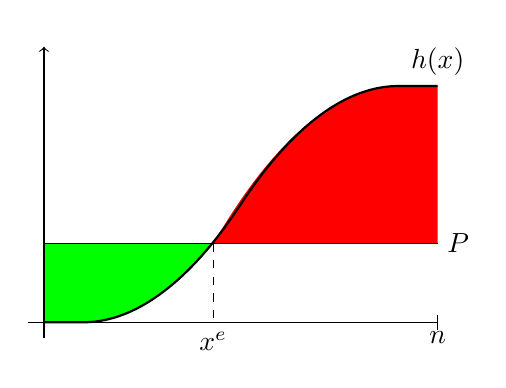
\begin{tikzpicture}[scale=1]
    \fill[green] (0,0) to (.5,0) parabola (2.15,1) to (0,1) to (0,0);
    \fill[red] (2.15,1) parabola[bend at end] (4.5,3) to (5,3) to (5,1) to (2,1);
    \draw[-|] (-0.2,0) -- (5,0) node[below]{$n$}; 
    \draw[->] (0,-0.2) -- (0,3.5) node[above]{};
    \draw[thick] (0,0) to (.5,0) parabola (2.5,1.5) parabola[bend at end] (4.5,3) to (5,3) node[above]{$h(x)$};

    \draw[thin] (0,1) to (5,1) node[right]{$P$};
    \draw[dashed, thin] (2.15,1) -- (2.15,0) node[below]{$x^e$}; 

%    \draw[thin] (0,2) to (5,2) node[right]{$S+P$};
%    \draw[dashed, thin] (1.75,1.5) -- (1.75,0) node[below]{$x^p$}; 
    
%    \draw[thin] (0,3) to (5,3) node[right]{$S+P+L$};
%    \draw[dashed, thin] (3.55,3) -- (3.55,0) node[below]{$x^e$}; 
    
\end{tikzpicture}
    \caption{Non-Speech Torts}
    \label{fig:nonspeech}
\end{figure}
The net benefit or harm to society from the factory's production at $x$ is given between the signed difference between $P$ and $h(x)$. Production in the green region, where $P > h(x)$ is net beneficial. Although there are harms from pollution, they are outweighed by the value of the corresponding widgets. Production in the red region, where $P < h(x)$, is net harmful. Here, the harms from pollution are worse than the value of the corresponding widgets; society would be better off if these widgets were not produced at all. If that the factory produces up to a level $\hat{x}$, social welfare will be given by:
\begin{equation}
\int_{0}^{\hat{x}} P - h(x) dx
\end{equation}
It is easy to see that the efficient outcome is when the factory produces just up to the threshold $x^e$ defined by $h(x^e) = P$. At $x_e$, all of the beneficial widgets and none of the harmful widgets are produced. The question is how to get there. Write $x^{\ast}$ for the production level that maximizes the factory's profits, and consider the following legal regimes:
\begin{itemize}
\item \textbf{No liability}: If the factory faces no liability for the pollution it causes, it will set $x^{\ast} = n$, making a profit of $nP$. But since $n > x^e$, social welfare will be less than the efficient level, and may even (as in the diagram above) be negative.
\item \textbf{Prohibition}: If society bans widgets, the factory will set $x^{\ast} = 0$ and make a profit of $0$. But since $0 < x^e$, social welfare will be less than the efficient level. For some values of $h$ and $P$, prohibition will be better than no liability; for other values, it will be worse.
\item \textbf{Strict Liability}: If the factory is forced to pay compensation for all of the harms that it causes, the factory's marginal profit will be $P - h(x)$, which is identical to the social welfare function. The factory's marginal profit will become zero at $x^e$, exactly when social welfare does. Thus $x^{\ast} = x^e$ and the factory will act efficiently.
\end{itemize}
This is the standard law-and-economics case for strict liability. But one of its essential assumptions fails when the product is not widgets, but speech.


\subsection{Model 2: Speech Liability}

Speech consists of information, and information is a public good. Once it has been shared with one listener, the speaker cannot easily prevent them from sharing it with others.\footnote{Arrow, Lemley, Frischmann, Baker} This third-party value is an externality from the speaker's perspective. We model it by adding an additional term $\delta > 0$ to the value created by carrying a given piece of content. Like $P$, we assume that $\delta$ is constant across all content. Thus, while each unit of widget production generates $P$ in marginal profit for the factory, each unit of speech generates $P$ in value for the speaker and $\delta$ in value for society at large, for a total of $P + \delta$. Again for simplicity, assume that $h(n) > P + \delta$. Now the diagram looks like:
\begin{figure}[h]
    \centering
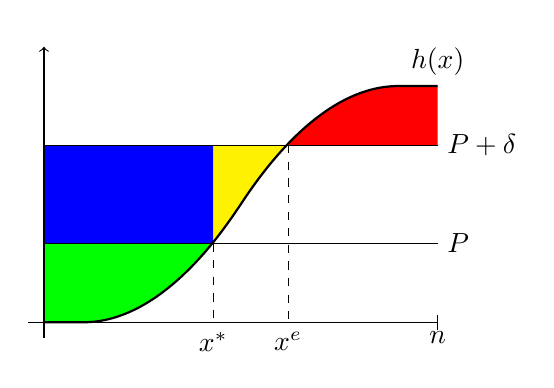
\begin{tikzpicture}[scale=1]
    \fill[green] (0,0) to (.5,0) parabola (2.15,1) to (0,1) to (0,0);
    \fill[red] (3.1,2.25) parabola[bend at end] (4.5,3) to (5,3) to (5,2.25) to (3.1,2.25);
    \fill[blue] (0,1) to (2.15,1) to (2.15,2.25) to (0,2.25) to (0,1);
    \fill[yellow] (2.15,1) parabola bend +(-1.65,-1) (2.5,1.5) parabola bend +(2,1.5) (3.1,2.25) to (2.15,2.25) to (2.15,1);
    \draw[-|] (-0.2,0) -- (5,0) node[below]{$n$}; 
    \draw[->] (0,-0.2) -- (0,3.5) node[above]{};
    \draw[thick] (0,0) to (.5,0) parabola (2.5,1.5) parabola[bend at end] (4.5,3) to (5,3) node[above]{$h(x)$};

    \draw[thin] (0,1) to (5,1) node[right]{$P$};
    \draw[dashed, thin] (2.15,1) -- (2.15,0) node[below]{$x^*$}; 

    \draw[thin] (0,2.25) to (5,2.25) node[right]{$P+\delta$};
    \draw[dashed, thin] (3.1,2.25) -- (3.1,0) node[below]{$x^e$}; 
    
%    \draw[thin] (0,3) to (5,3) node[right]{$S+P+L$};
%    \draw[dashed, thin] (3.55,3) -- (3.55,0) node[below]{$x^e$}; 
    
\end{tikzpicture}
    \caption{Speech Torts}
    \label{fig:nonspeech}
\end{figure}
The efficient level of speech $x^e$ is defined not by where $h(x)$ intersects the speaker's marginal profit curve $P$ but by where it intersects society's marginal benefit curve $P+\delta$. Under no liability, the speaker will still overproduce (producing the net-harmful speech in the red area); under prohibition, the speaker will still underproduce (failing to produce the net-beneficial speech in the green and blue areas) . But now also strict liability gets the incentives wrong. Under strict liability, the speaker will produce speech up to $x^*$ where $h(x^*) = P$. But because $P + \delta > P$ and $h(x)$ is a weakly increasing function, $x^* \le x^e$. Pictorially, the platform will produce up to $x^*$, generating profits in the green region and spillover social benefits in the blue region. But there it will stop, even though the speech from $x^*$ to $x^e$ would have been beneficial to society: the yellow region represents foregone social welfare. \footnote{Strict liability is strictly better than prohibition, which also gives up the green and blue regions. Whether strict liability is better than full immunity is indeterminate without more constraints on $h(x)$, $P$, and $\delta$; the yellow region could be larger than the red, or vice versa.}

Instead, free speech law typically follows the negligence strategy of defining an objective standard of care that a reasonable person is expected to follow when acting. One who acts according to that standard of care faces no liability, even if others are harmed. But one who fails to meet that standard is held liable for the resulting harms. In our model, this approach corresponds to defining a threshold of liability $t$ and subjecting the actor to marginal liability:
\begin{equation}
\lt\{\begin{array}{ll}
    0 & \mbox{for $x <t$}, \\
    h(x) & \mbox{for $x \ge t$}.
\end{array}\rt.
\end{equation}
It is easy to see that if the threshold is set at $t=x^e$, then the actor's incentives again align with social welfare.\footnote{Cooter, prices and sanctions} This is a standard argument for treating speech torts differently than other types of torts. Because the speaker creates value for listeners and for society by spreading information, the value of the speech \emph{to them} must be weighed against the harm that it causes. Thus, harmful true speech is frequently protected (e.g. negative consumer reviews). Similarly, the public-disclosure tort contains a First-Amendment-driven exception when the information is of legitimate public concern, i.e., when $\delta$ is high.

This model explains why speech law is more solicitous of speakers than of other actors. But notice that it cannot yet explain why speech law is even more solicitous of platforms than it is of speakers! The spillover critique of strict liability applies just as strongly to original speakers as it does to platforms. And the negligence strategy suggests that the threshold of liability should be based entirely on the overall \emph{social} costs and benefits of the speech: whatever that threshold is, it should apply equally to speakers and platforms, regardless of their private incentives. Something further is required to make sense of platform immunity.




\subsection{Model 1: Beneficial and Harmful Content}

Users of a platform submit some large number of items of content. Each of these items generates some value for the speaker who posted it, for the platform, and for its listeners. It also potentially generates some harms for third parties: copyright infringement harms copyright owners, defamation harms the defamed, and so on. We are interested in the platform's responses to content of varying harmfulness, so we treat the benefits as fixed parameters and the harms as variable. We can model how the platform's responses change for different categories of content by changing the parameters.

The users of the platform submit some large number $n$ of items of content. Let the variable $x \in [0,n]$ range over the content. For each $x$, the platform has the option either to leave it up or to take it down. If the platform leaves it up, there are four effects:
\begin{itemize}
\item It generates fixed value $S \ge 0$ for the speaker who posted it.
\item It generates fixed value $P \ge 0$ for the platform.
\item It generates fixed value $L \ge 0$ for the listeners who read it, and for others in society.
\item It causes variable harm $h(x)$ for other members of society.
\end{itemize}
Although technically each item is discrete, for simplicity we treat the range $[0,n]$ as a continuum, so that $x$ and any functions of $x$ are continuous.\footnote{In the  case of a large platform, where the number of individual items is enormous, in the millions or even billions, a continuous approximation is quite reasonable.} We also assume that the items are ordered by increasing harmful harmfulness, so that $h(x)$ is a weakly increasing function of $x$. That is, if $x < y$, then $h(x) \le h(y)$. We also assume that the least harmful content is completely harmless, i.e. $h(0) = 0$. The following diagram illustrates for the case when the most harmful content is unambiguously harmful, i.e.  $h(n) > S + P + L$:

\begin{figure}[h]
    \centering
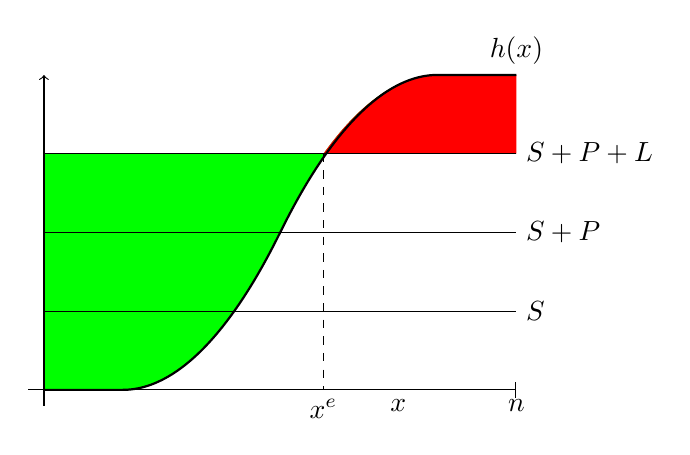
\begin{tikzpicture}[scale=1]
    \fill[green] (0,0) to (1,0) parabola (3,2) parabola bend +(2,2) (3.55,3) to (0,3) to (0,0);
    \fill[red] (3.55,3) parabola[bend at end] (5,4) to (6,4) to (6,3) to (3.55,3);
    \draw[-|] (-0.2,0) -- (3,0) -- node[below]{$x$} (6,0) node[below]{$n$}; 
    \draw[->] (0,-0.2) -- (0,4) node[above]{};
    \draw[thick] (0,0) to (1,0) parabola (3,2) parabola[bend at end] (5,4) to (6,4) node[above]{$h(x)$};

    \draw[thin] (0,1) to (6,1) node[right]{$S$};
%    \draw[dashed, thin] (1.75,1.5) -- (1.75,0) node[below]{$x^s$}; 

    \draw[thin] (0,2) to (6,2) node[right]{$S+P$};
%    \draw[dashed, thin] (1.75,1.5) -- (1.75,0) node[below]{$x^p$}; 
    
    \draw[thin] (0,3) to (6,3) node[right]{$S+P+L$};
    \draw[dashed, thin] (3.55,3) -- (3.55,0) node[below]{$x^e$}; 
    
\end{tikzpicture}
    \caption{Social benefits and harms of content}
    \label{fig:removal}
\end{figure}


The net benefit or harm to society of the content on the platform is given by the signed difference between $h(x)$ and $S+P+L$. The green region represents the content that is net beneficial, i.e. $S+P+L > h(x)$. The red region represents the content that is net harmful, i.e. $h(x) > S+P+L$. The diagram shows that there is a unique efficient outcome defined by setting a threshold $x^e$ defined by $h(x^e) = S + P + L$, in which all of the net beneficial content (with $x < x^e$) stays up and all of the net harmful content (with $x > x^e$) is removed.

In a standard tort-liability model, an actor chooses a level of activity that causes both private benefits and harms to identifiable victims. A regime of strict liability, in which the actor must compensate the victims for the harms they suffer, leads to an efficient outcome. And if there were a single actor that realized the full social value $S + P +L$ from the content $x$ that it leaves up, a strict liability regime requiring it to pay compensation $h(x)$ for the harms caused by that content would be efficient. 

In our model, this is the case when the platform captures all of 





% Figure here with constant P

The shaded area is the total value to users of posting their content to the platform. It has height $P$ and width $N$, for total value $PN$. This the value to users of having the platform, if it were free to them.

Now, consider the platform's incentives. For now, we assume that the platform can capture all of the value to users of posting their content. We also assume that the platform has infinite capacity, but incurs fixed costs $F$, which it must pay to operate all. Then the platform's profit if it operates is $PN - F$. The following diagram shows the platform's profits if it operates as a function of $N$.

% Diagram

It starts at $-F$ and crosses the $x$ axis at $N = F/P$. Beneath that level, the platform is unprofitable and will not operate at all, so that the value to society is $0$. Above that level, the platform recovers its costs and hosts all the content, so that the value to society is $PN - F $.(We must of course include the costs of operating the platform in the 

Because the platform captures all of the users' value, it fully internalizes all of the costs and benefits to society of operating. Thus, society's overall welfare function is the same as the platform's profits. If $PN < F$, the platform is a net negative because it costs more to operate than the value it delivers, and a regulator should prefer that it not operate. If $PN > F$, the platform is a net positive and a regulator should prefer it to operate. No regulation is required; the platform's incentives match the regulator's goals.

\subsection{Model 2: Harmful Content}
 
Now we consider the fact that some content is harmful. Suppose that \emph{some} of the items of content cause constant harm $H$ if the platform hosts them. In this model, we assume that everyone (including the regulator and the platform) knows which items these are. Thus, without loss of generality, \emph{we order the items of content by how harmful they are, from least harmful to most harmful}. Since the harm cause by harmful content is constant, this means we can define a step function $h(x)$:

\begin{equation}
h(x)=
\lt\{\begin{array}{ll}
    0 & \mbox{if $x>\hat{x}$}, \\
    H & \mbox{otherwise}.
\end{array}\rt.
\end{equation}

In the case where $H>P$, each item of harmful content is a net negative for society. This results in the following diagram:

% Step function h

The shaded area on the left, with area $\hat{x}P$, consists of the beneficial content. The shaded area on the right, with area $(N - \hat{x})(H-P)$, consists of the harmful content. The socially efficient outcome is achieved when the platform hosts only the beneficial content.

We introduce new notation for the idea that the platform can set a threshold: for $x$ beneath the threshold, the platform leaves the content up, for $x$ greater than the threshold, the platform takes the content down. We define $x^e$ (the $e$ is for ``efficient'') to be the cutoff point at which the threshold is efficient. It is obvious by inspection that in this model $x^e = \hat{x}$ -- subject to the same condition as above, that it is efficient for the platform to operate at all. If $\hat{x}P < F$, the game is not worth the candle, and society prefers that the platform not operate at all. Otherwise, social welfare is $\hat{x}P - F$.

Now consider the platform's incentives, which can diverge from the regulator's goals because the platform internalizes $P$ (the value of content to users) but not $H$ (the harm caused by the content).  In the absence of liability, the platform will host \emph{all} the content, beneficial and harmful, for net profits of $NP - F$, as above. But now social welfare equals $\hat{x}P - F - (N - \hat{x})(H - P)$, which is smaller than the social welfare at $x^e$ because of the extra term.

What should the regulator do? One option is to prohibit all platforms. This is an improvement on the no-regulation baseline in the case where $\hat{x}P - (N - \hat{x})(H - P) - F < 0$. But it is not efficient in the case where $\hat{x}P > F$, and it would be profitable to have  platform operate.

Instead -- and this is the classic starting point of law-and-economics analysis of tort liability -- the regulator should impose liability on the platform for the harmful content it carries. This fixes the platform's incentives by making it internalize both the costs and the benefits of its conduct. One rule, of strict liability, holds the platform liable for all the harm it causes. Under this rule, for $x <\hat{x}$, the platform has marginal profit of $P$, which is positive, so it will add more content until it reaches $\hat{x}$. But for $x > \hat{x}$, the platform's marginal profit is $P - H$, which is negative, so it will remove content until it reaches $\hat{x}$.  Introducing the notation $x^*$ for the platform's optimum, we say that $x^* = x^e = \hat{x}$.

Another classic rule, of negligence, sets a level of care $x^n$ and imposes liability $L$ for each item of content if the platform operates above that level. But here, the efficient level of care is just $x^n = \hat{x}$ again, so as long as $L>P$, the platform will again set its threshold at the efficient point of $\hat{x}$ and the two rules are effectively identical.

Before moving on, consider another variation in the parameters. We have been discussing the case where $H > P$. But there is also the case where $H < P$ -- i.e., the content is beneficial on net, but causes harms the platform does not internalize.

% diagram

Here, the efficient level of operation is $x^e = N$, i.e. society prefers that all of the content remain available. Under the no-liability baseline, the platform will do just that. But if the regulator imposes liability, matters are more complicated. If the platform must pay compensation $H$ for each item of harmful content, its profits are $NP - (N - \hat{x})(P - H) - F $. This can cause the platform to shut down if the need to pay compensation makes it unviable, i.e., when 

\begin{equation}
NP - (N - \hat{x})(P - H) < F <  NP
\end{equation}

% Diagram platform's profits as a function of $x^c$.

This concern puts regulators to a choice: in some cases, \emph{without the profits attributable to harmful content, a platform cannot operate to serve beneficial content}. In this model with $H < P$, the problem is avoidable, because even the content that causes harms is still beneficial on net. But we will soon see models in which the tradeoff is sharper.


\subsection{Model 3: Variably Harmful Content}

In the previous model, $h(x)$ was a step function: some content is harmless with $h(x) = 0$ and some content is harmful with $h(x) = H$. Now we extend this model by making $h(x)$ a more general function. Once again, we order the content by increasing harmfulness, so that $h(x) \le h(y)$ for $x < y$. We also assume that $h(0) =0$ (i.e., there is some content that is unambiguously good). To simplify the case analysis, we also require that $h(N) => P$, i.e. there is some content that is unambiguously harmful. Now the diagram of the benefits and harms from content looks like the following:

% diagram

The regulator would prefer the content to carry all content $x$ for which $h(x) <P$ and to remove all content for which $h(x) > P$. By the intermediate value theorem, there is some point $x^e$ for which $h(x^e) = P$. Because $h(x)$ is weakly increasing, it follows that $h(x) \le P$ for all $x< x^e$ and $h(x) \ge P$ for all $x > x^e$. Thus, the same result as in the previous model follows: the regulator wants the platform to allow content exactly up to $x = x^e$. The actual expression for social welfare is more complicated because $h(x)$ is no longer constant. If the platform leaves up all content through $\hat{x}$, then the social welfare function is

\begin{equation}
\int_{0}^{\hat{x}} P - h(x) dx - F
\end{equation}

In the absence of liability, however, the platform fails to internalize the harms. Its profit function is 

\begin{equation}
\int_{0}^{\hat{x}} P dx - F
\end{equation}

which it maximizes by setting $\hat{x} = N$, i.e. leaving up all content. Once again, the regulator can impose strict liability. If it does so, then the platform's profit function equals the social welfare function, and the platform will set the efficient threshold $\hat{x} = x^e$. Similarly, the regulator could impose a threshold-based liability $h(x)$ starting at at threshold $x^n$. In this case, the platform's marginal profit will be $P$ for $x < x^n$ and $P - h(x)$ for $x > x^n$, and the platform has efficient incentives for $x^n = x^e$. 

The difference between the two regimes is that in the former, the platform compensates those who are harmed for $x < x^e$; in the latter it does not. In diagram XXX, this compensation is the difference between the two shaded regions 1 and 2, and just the upper one. In the case where

XXX equation

the choice can affect the viability of the platform, just as in the previous model.

\subsection{Model 4: Positive Externalities}

Next, we add in another important fact about content: it creates positive externalities that are not fully captured by the platform. There are several overlapping reasons why this is so:

\begin{itemize}
\item The platform may not be able to price access in ways that captures all of the surplus it creates for its users.
\item Information is a public good. Once it has been shared on the platform, it can be shared further in ways the platform cannot perfectly track or monetize.
\item A typical platform has at least some competition, so it will price beneath the level it would as a monopolist.
\end{itemize}

We model these externalities by adding an additional term $\delta$ to the value created by carrying a given piece of content. Like $P$, we assume that $\delta$ is constant across all content. Thus, each piece of content carried generates $P$ in value for the platform and $\delta$ in value for society at large, for a total of $P + \delta$. Again for simplicity, assume that $h(N) > P + \delta$. Now the diagram looks like:

% diagram with P, P + \delta, and h(x)

Assuming the platform operates, the efficient level of moderation is at $x^e$ where $h(x^e) = P + \delta$. With immunity, the platform undermoderates, just as before, and hosts all content. Under strict liability, the platform moderates at $x^*$ such that $h(x^*) = P$, which is to the left of $x^e$, i.e., the platform undermoderates. The shaded triangle in diagram XXX illustrates the lost social value: this is content that is positive-value for society (because $h(x) < P + \delta$ but which is unprofitable for the platform to host (because $h(x) > P$). Compare the result under a threshold liability rule: the regulator will set the threshold at $x^e$ rather than at $x^e$, leading the platform to set its cutoff at $x^e$.




\subsection{Model 5: Unknown Content}

All of the previous models assumed perfect information about the harms caused by content. It is time to relax this assumption, because several of the most interesting and important consequences for content moderation depend on the difficulty of distinguishing between beneficial and harmful content.

We return to a fixed harm: each item of harmful content causes harm $H$. But now we make the \emph{probability} of harm variable. The function $\lambda(x)$ represents the probability that the item of content $x$ is harmful. That is, with probability $\lambda(x)$, item $x$ causes harm $H$, and with probability $1 - \lambda(x)$, it causes harm $0$. We assume that the platform and regulator have perfect information about $H$ and $\lambda()$, that $\lambda(x)$ is weakly increasing in $x$, and that there is some content known to be harmless and some known to be harmful, i.e. $\lambda(0) = 0$ and $\lambda(N) = 1$. The following diagram illustrates:

% diagram

This diagram should look familiar. It is the same as diagram XXX, except that the harm curve is now labeled $\lambda(x)H$ rather than $h(x)$. But the shape of the curves are the same. Each individual piece of content $x$ is either harmful or not with probability $\lambda(x)$, but in the continuous limit of an infinitely large $H$, this is the same as if the content in the neighborhood of $x$ is all equally harmful with harm $\lambda(x)$.

In particular, the regulator and platform have exactly the same welfare and utility functions as before.  If the platform leaves up all content through $\hat{x}$, then the social welfare function is

\begin{equation}
\int_{0}^{\hat{x}} P - \lambda(x)H dx - F
\end{equation}

so that social optimum where the marginal harm and marginal benefit from additional content exactly cancel is at $x^e$ such that $P = \lambda(x^e)H$. As before, however, the platform's profit function in the absence of liability is

\begin{equation}
\int_{0}^{\hat{x}} P dx - F
\end{equation} 

which is again maximized for $\hat{x} = N$. The same argument as above shows that either strict liability for all harms caused or liability for all harmful content above the threshold $x^e$ is efficient -- subject to the constraint that in the former case the platform must be profitable, i.e. $\int_0^{x^e} P dx = x^eP \ge F$.


\subsection{Model 6: Platform Investigation}

The next model is the same as the previous one -- content causes harm $H$  with weakly increasing probability $\lambda(x)$ -- except that the platform now has a new option. It can incur a cost of $c > 0$ to investigate an item of content and determine with certainty whether it is harmful. Note that it only makes sense for the platform to investigate if the results will affect the platform's decision. Otherwise, the platform could save $c$ by skipping the investigation and doing what it would have done anway.

If the platform operates at all, then, it has three options for any given item of content: it can leave it up, take it down, or investigate -- where it will take the content down if the investigation reveals it to be harmful, and leave it up otherwise. Thus the expected value to society for a given $x$ is $0$ if the platform takes down the content, $P + \delta - \lambda(x)H$ if it leaves the content up, and $(P + \delta)(1 - \lambda(x)) - c$ if it investigates -- i.e., the value of a non-harmful piece of content times the probability that the content is non-harmful. Intuitively, the platform should prefer takedown for content with $\lambda(x)$ close to $1$ and should prefer leaving up for content with $\lambda(x)$ close to $0$, with an interval of investigation somewhere in the middle. The following diagram illustrates:

% diagram

The regulator is indifferent between takedown and investigation when $(P + \delta)(1 - \lambda(x)) - c = 0$, which is the case when $\lambda(x) = 1 - \frac{c}{P + \delta}$. When $c$ approaches $0$, this converges to $\lambda(x) = 1$, i.e., so the right end of the investigation interval approaches $N$. That is, it is almost always better to investigate than to take down the content without first checking. And when $c$ is greater than $P+\delta$, it is the case that $\lambda(x) <0$, i.e. it is never worth investigating rather than simply taking down the content because the game is not worth the candle.

The regulator is indifferent between investigation and leaving up when $(P + \delta)(1 - \lambda(x)) - c = P + \delta - \lambda(x)H$, which is the case when $\lambda(x) = \frac{c}{H - P - \delta}$. Again, limiting cases show the behavior clearly. When $c$ approaches $0$, this converges to $\lambda(x) = 0$, i.e., the left end of the investigation interval approaches $0$. That is, it almost always better to investigate than to leave up the content without first checking. Contrariwise, when $c > H - P - \delta$, it is never worth investigating.

These two results show that a rational regulator should want platforms to invest resources in investigating only a range of intermediate cases where the harmfulness of the content is sufficiently unclear. For content that is highly likely or highly unlikely to be harmful, individual investigation is unnecessary and inefficient. In notation, we can say that the efficient range of investigation is $[\underline{x}^e, \overline{x}^e$, where the lower limit  is given by $\lambda(\underline{x}^e) = \frac{c}{H - P - \delta} $ and the upper limit by $\lambda(\overline{x}^e) = 1 - \frac{c}{P + \delta}$.

What the \emph{platform} will do, however, is more complicated. Start with the case of strict liability, where the platform internalizes all the harm that it causes. The platform's profit for item $x$ is the same as the overall social value, except without the $\delta$ term for the uninternalized spillover benefits. Thus its interval of investigation is $[\underline{x}^*, \overline{x}^*$, where the lower limit  is given by $\lambda(\underline{x}^*) = \frac{c}{H - P} $ and the upper limit by $\lambda(\overline{x}^*) = 1 - \frac{c}{P}$.

The key result is that the platform's preferred interval of investigation is always \emph{narrower} than the regulator's preferred interval. (Algebraically.this is because  $\frac{c}{H - P - \delta} < \frac{c}{H - P}$ at the lower end and $1 - \frac{c}{P} < 1 - \frac{c}{P + \delta}$ at the upper end.) Intuitively, because the platform has less at stake, it is less willing to expend effort to separate sheep from goats, and will be comfortable with more approximate strategies for content that looks sufficiently harmful or harmless. The following diagram illustrates:

% diagram